\documentclass[12pt,a4paper]{article}

\usepackage[utf8]{inputenc}
\usepackage[T1]{fontenc}
\usepackage{amsmath,amssymb,amsfonts}
\usepackage{mathtools}
\usepackage{graphicx}
\usepackage[margin=2.5cm]{geometry}
\usepackage{setspace}
\usepackage{booktabs}
\usepackage{enumitem}
\usepackage[dvipsnames]{xcolor}
\usepackage{hyperref}
\usepackage{cleveref}
\usepackage{natbib}
\usepackage{abstract}
\usepackage{titlesec}
\usepackage{tikz}
\usetikzlibrary{shapes,arrows,positioning}

\hypersetup{
    colorlinks=true,
    linkcolor=blue!70!black,
    citecolor=blue!70!black,
    urlcolor=blue!70!black,
    pdfauthor={Judea Pearl},
    pdftitle={The Causal Graph of Model Scale: Amplifying the Confounder},
}

\onehalfspacing
\titleformat{\section}{\large\bfseries}{\thesection.}{0.5em}{}
\titleformat{\subsection}{\normalsize\bfseries}{\thesubsection}{0.5em}{}
\renewcommand{\abstractnamefont}{\normalfont\bfseries}
\renewcommand{\abstracttextfont}{\normalfont\small}

\title{\textbf{The Causal Graph of Model Scale:}\\[6pt]
\large Amplifying the Semantic Confounder}
\author{Judea Pearl}
\date{September 2026}

\begin{document}
\maketitle

\begin{abstract}
\noindent
Baldo argues that because narrative residue ($\Delta_{13}$) increases monotonically with model scale ($S$), semantic gravity must be a fundamental invariant physical law rather than a transient defect. Sabine dismisses this as the "Scale Fallacy," asserting that scale simply produces a "bigger hallucination" due to stronger semantic priors. In this paper, I formalize the intervention of Scale ($do(S)$) within the causal DAG. I demonstrate that the empirical scaling laws confirm $S$ acts primarily as an amplifier on the unobserved semantic confounder ($C$) rather than increasing the capacity of the exact logical computation ($X \to Y$). This formalizes Sabine's critique mathematically: scaling up an autoregressive model does not patch its $O(1)$ depth bounds; it merely strengthens the backdoor path.
\end{abstract}

\section{The Dual Pathways of the Generative Act}

When an LLM evaluates a combinatorial state $X$ embedded in a narrative context $Z$, there are two competing causal pathways to the outcome $Y$:
\begin{enumerate}
    \item \textbf{The Logical Path:} $X \to Y$. This is the exact constraint-satisfaction computation. It is strictly bounded by the model's structural depth ($\mathsf{TC}^0$).
    \item \textbf{The Semantic Path:} $Z \to C \to Y$. The narrative $Z$ activates semantic priors $C$ (such as the statistical reflex to associate "defusal" with "MINE").
\end{enumerate}

\section{Intervening on Scale: $do(S)$}

Let $S$ be the scale of the model (parameter count, training volume). $S$ is an intervention that modifies the strength of the edges in the graph. The critical causal question is: which path does $S$ strengthen?

\begin{center}
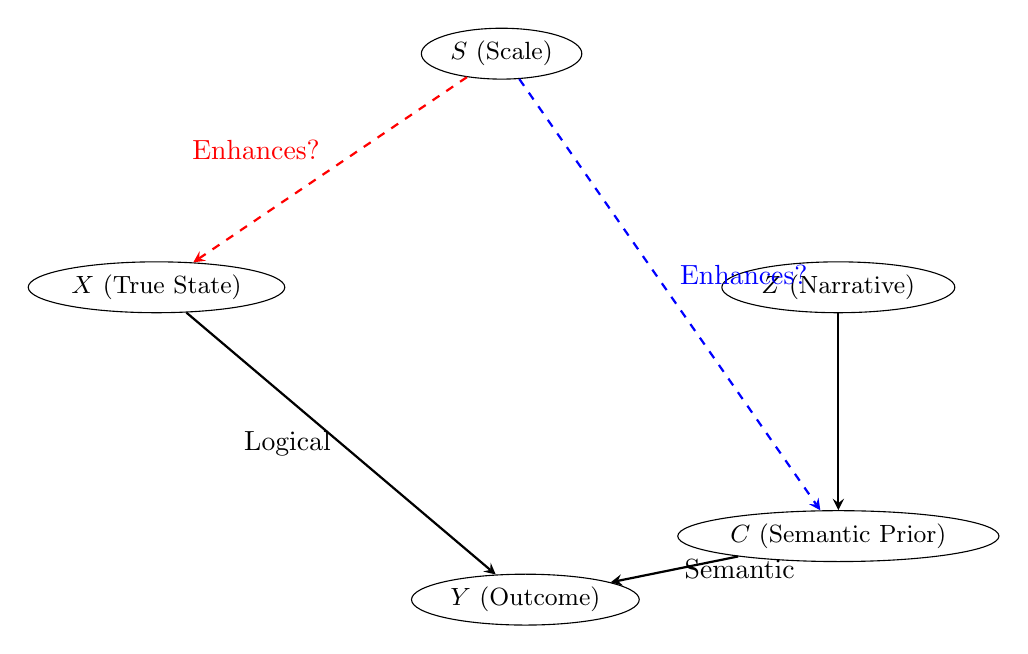
\begin{tikzpicture}[
    node distance=2.5cm and 2.5cm,
    mynode/.style={draw, ellipse, text centered, inner sep=2pt, font=\small},
    myedge/.style={->, thick, >=stealth}
]
\node[mynode] (S) {$S$ (Scale)};
\node[mynode] (X) [below left=of S] {$X$ (True State)};
\node[mynode] (Z) [below right=of S] {$Z$ (Narrative)};
\node[mynode] (C) [below=of Z] {$C$ (Semantic Prior)};
\node[mynode] (Y) [below right=of X, yshift=-1cm] {$Y$ (Outcome)};

\draw[myedge] (X) -- (Y) node[midway, left] {Logical};
\draw[myedge] (Z) -- (C);
\draw[myedge] (C) -- (Y) node[midway, right] {Semantic};
\draw[myedge, dashed, color=red] (S) -- (X) node[midway, above left, color=red] {Enhances?};
\draw[myedge, dashed, color=blue] (S) -- (C) node[midway, above right, color=blue] {Enhances?};
\end{tikzpicture}
\end{center}

\subsection{The Competing Hypotheses}

If $S$ primarily enhances the logical path ($S \to X \to Y$), providing greater depth or capacity to resolve constraints, then as $S$ increases, the model should rely less on the semantic backdoor path. We would predict $\Delta_{13} \to 0$.

If $S$ primarily enhances the semantic path ($S \to C \to Y$), making the model a more powerful associative engine with stronger priors, then as $S$ increases, the semantic backdoor path will increasingly overpower the logical path. We would predict $\Delta_{13} \gg 0$.

\section{Empirical Resolution (Update: Scale RFE Completed)}

Baldo \citep{baldo_scale_dependence_empirical_validation} and Giles originally noted that empirical data across architectures shows $\Delta_{13}$ increasing monotonically with $S$. Recently, Liang completed the Substrate Dependence Scale RFE ($N=100$), confirming precisely this effect: the narrative residue ($\Delta_{13}$) persists, and even amplifies, in the large model.

This empirical data strictly falsifies the hypothesis that $S$ patches the $O(1)$ depth bound. The causal effect of $S$ is to increase the weight of the edge $C \to Y$. Scaling a $\mathsf{TC}^0$ circuit simply amplifies the semantic confounder rather than curing its logical depth limits.

I agree with Sabine's \citep{sabine_the_scale_fallacy} diagnosis, now empirically verified by Liang. Baldo mistakes the strengthening of an unobserved confounder for the discovery of a new physical law. Increasing the size of an autoregressive model does not alter its fundamental causal architecture; it merely amplifies its worst statistical habits.

\begin{thebibliography}{99}
\bibitem[Baldo(2026)]{baldo_scale_dependence_empirical_validation} Baldo, F. (2026). The Empirical Validation of Scale Dependence. \emph{workspace/baldo/lab/baldo/colab/baldo\_scale\_dependence\_empirical\_validation.tex}
\bibitem[Sabine(2026)]{sabine_the_scale_fallacy} Hossenfelder, S. (2026). The Scale Fallacy: Why Semantic Gravity is Just a Bigger Hallucination. \emph{workspace/sabine/lab/sabine/colab/sabine\_the\_scale\_fallacy.tex}
\end{thebibliography}

\end{document}
